\chapter{Cónicas y Cuádricas}
\label{C8}
A lo largo del capítulo $\ref{C2}$ estudiamos con detalle el conjunto de puntos que eran anulados por unas aplicaciones muy concretas, a las que llamamos \ti{formas lineales}.

En este capítulo haremos algo parecido, dando un pequeño paso adelante, pues estudiaremos las interesantes propiedades del conjunto de ceros de las llamadas \ti{formas cuadráticas}.

A no ser que establezcamos explícitamente lo contrario, a lo largo de este capítulo trabajaremos con el cuerpo de los números complejos y el plano proyectivo complejo $\proy(\C^3)=\proy^2$. 

Esto es debido a que, como se verá inmediatamente, trabajaremos con polinomios, siendonos muy útil la posibilidad de aplicar el Teorema Fundamental del Álgebra y sus consecuencias.

El capítulo comienza con una fuerte introducción teórica acerca de formas bilineales y cuadráticas (muy susceptible de haber sido olvidada), e indispensable para comprender en profundidad los resultados centrales del capítulo (razón por la cual se ha decidido incluirla aquí y no en un apéndice dedicado).

\section{Conceptos Previos. Formas Bilineales y Cuadráticas}
A lo largo de este capítulo estudiaremos las llamadas \ti{cuádricas}. Para poder definir de forma rigurosa este concepto, necesitamos recordar (o introducir) algunas nociones importantes más propias del álgebra lineal.
\subsection{Formas Bilineales}
Sea $E$ un espacio vectorial arbitrario de dimensión $n$. (Normalmente trabajaremos con $\C^n$).
\begin{defi}[Forma Bilineal]
	\label{C8_def_formaBilineal}
	Llamamos \ti{formas bilineales} a las aplicaciones de la forma \[\begin{array}{cc}f:&E\times E\to\K\\
	& (u,v)\mapsto f(u,v)\end{array}\]
	Donde $f$ es ``lineal respecto de ambas componentes''. Es decir, dado un par $(u,v)\in E\times E$, se verifica:
	\begin{enumerate}
		\item Linealidad respecto de la primera componente: \[f(\alpha u_1,\beta u_2, v)=\alpha f(u_1,v)+\beta f(u_2,v)\]
		\item Linealidad respecto de la segunda componente:
		\[f(u,\alpha v_1 +\beta v_2)=\alpha f(u,v_1)+\beta f(u,v_2)\]
	\end{enumerate}
\end{defi}
En este punto es fructífero recordar que una aplicación lineal queda totalmente determinada por las imágenes de los vectores de una base de su espacio vectorial de partida.

Este resultado daba lugar a la idea caracterizar cada aplicación lineal $f$ por una matriz, a la que llamábamos \ti{matriz asociada a $f$}.

Tratemos de trasladar esta idea al ámbito de las formas bilineales.
\subsubsection{Matriz Asociada a una Forma Bilineal}
Fijemos una base $\mc{B}:=\{e_1,\dots,e_n\}$ del espacio vectorial $E$.

Veamos cuál es la imagen del par $(u,v)$ por una forma bilineal arbitraria $f$. Para ello, escribiremos los vectores $u$ y $v$ como combinación lineal de la base $\mc{B}$ y aplicaremos las propiedades de bilinealidad (definición \ref{C8_def_formaBilineal})
\[f(u,v)=f\left(\sum_{i=1}^{n}a_ie_i,\sum_{j=1}^{n}b_je_j\right)=\sum_{i=1}^{n}a_i\left(\sum_{j=1}^{n}f(e_i,e_j)b_j\right)\]
Podemos interpretar el interior del paréntesis como un producto de matrices (matriz fila por matriz columna). Haciendo esto obtenemos la siguiente expresión, más compacta (los corchetes son sólo notacionales).
\[f(u,v)=\sum_{i=1}^{n}a_i\left[\begin{pmatrix}
f(e_i, e_1) & 
\cdots &
f(e_i, e_n)
\end{pmatrix}\begin{pmatrix}
b_1 & \cdots & b_n
\end{pmatrix}^t\right]\]
Por comodidad notacional, a la matriz columna que representa las coordenadas de $v$ respecto de $\mc{B}$ será denotado por $Y$. Análogamente, llamaremos $X$ a la matriz columna que representará las coordenadas de $u$ respecto de $\mc{B}$.

Con esta notación (y reordenando por conveniencia los corchetes) nos queda:
\[f(u,v)=\left[\sum_{i=1}^{n}a_i\begin{pmatrix}
f(e_i, e_1) & 
\cdots &
f(e_i, e_n)
\end{pmatrix}\right]Y\]
Como hicimos antes, podemos interpretar la suma anterior de manera matricial (las comprobaciones de dejan al lector)
\[f(u,v)=\begin{pmatrix}
a_1 & \cdots & a_n
\end{pmatrix}\begin{pmatrix}
f(e_1, e_1) & \cdots & f(e_1,e_n)\\
\vdots & \ddots & \vdots\\
f(e_n,e_1) & \cdots & f(e_n,e_n)
\end{pmatrix}Y\]
Usando nuestras notaciones habituales y denotando por $M$ a la matriz cuadrada obtenemos:
\begin{equation}
\label{C8_eq_ecuacionMatricialBilineal}
f(u,v)=X^tMY
\end{equation}
A la matriz $M$ de la ecuación \eqref{C8_eq_ecuacionMatricialBilineal} se la llama \ti{matriz asociada a la forma bilineal $f$}.

Se ve inmediatamente por la ecuación \eqref{C8_eq_ecuacionMatricialBilineal} que si dos formas bilineales $f$ y $g$ tienen a $M$ por matriz asociada, estas son necesariamente la misma aplicación.

Esto quiere decir que una forma bilineal $f$ queda totalmente determinada por su matriz asociada, es decir, por las imágenes de los pares de vectores $(e_i,e_j)$ donde $i,j\in\{1,\dots,n\}$.

\begin{obs}[Lema de la Correspondencia]
	\label{C8_obs_correspondencia}
	Es claro que a lo largo de este proceso hemos probado que, \tb{fijada una base} $\mc{B}$ de $E$, toda forma bilineal $f$ está asociada a una única matriz $M$.
	
	Además, el recíproco también es cierto, fijada una base, toda matriz cuadrada es la asociada de una única forma bilineal.
	
	La prueba de este hecho consiste símplemente en definir una forma bilineal $f$ de manera que la imagen de un par de la forma $(e_i,e_j)$ se corresponda con el coeficiente $a_{ij}$ de la matriz dada. 
\end{obs}
\subsection{Formas Cuadráticas}
Introducidos ya los aspectos generales de las formas bilineales, pasemos a definir la noción de \ti{forma cuadrática}.
\begin{defi}[Forma Cuadrática]
	Una aplicación $\Phi$ se dice \ti{forma cuadrática} si es de la forma:
	\[\begin{array}{cc}
	\Phi: & E\to \K\\
	& x\mapsto f(x,x)
	\end{array}\]
	donde $f$ es una forma bilineal.
\end{defi}
Es claro que, fijada una base, las formas cuadráticas cumplen la siguiente ecuación matricial:
\begin{equation}
\label{C8_eq_ecuacionCuadraticas}
	\Phi(x)=X^tMX
\end{equation}
Una propiedad agridulce de las formas cuadráticas es que pueden estar asociadas a varias formas bilineales, tal y como muestra el siguiente ejemplo.
\begin{exa}[Varias Formas Bilineales Asociadas]
	Sean las formas bilineales de matrices asociadas:
	\[f\equiv\begin{pmatrix}
	1 & 4\\
	2 & 2
	\end{pmatrix}\qquad g\equiv\begin{pmatrix}
	1 & 3\\
	3 & 2
	\end{pmatrix}\]
	Comprobemos que ambas formas bilineales tienen la misma forma cuadrática asociada.
	\[\Phi_f(x)=\begin{pmatrix}
	x_1 & x_2
	\end{pmatrix}\begin{pmatrix}
	1 & 4\\
	2 & 2
	\end{pmatrix}\begin{pmatrix}
	x_1\\
	x_2
	\end{pmatrix}=x_1^2+6x_1x_2+2x_2^2\]
	\[\Phi_g(x)=\begin{pmatrix}
	x_1 & x_2
	\end{pmatrix}\begin{pmatrix}
	1 & 3\\
	3 & 2
	\end{pmatrix}\begin{pmatrix}
	x_1\\
	x_2
	\end{pmatrix}=x_1^2+6x_1x_2+2x_2^2\]
\end{exa}
Decimos que esta propiedad es ``agridulce'', porque por una parte es más bonito que haya una correspondencia ``limpia'' entre formas bilineales y formas cuadrátricas. Sin embargo, las propiedades que vienen a continuación compensan con creces esto último. Antes de poder presentarlas, necesitamos una pequeña definición.
\begin{defi}[Formas Bilineales Simétricas y Antisimétricas]
	\label{C8_def_simetricaAntisimetrica}
	Decimos que una forma bilineal $f$ es \ti{simétrica} si su matriz asociada es simétrica. Análogamente, $f$ será \ti{antisimétrica} (o \ti{alternada}) si su matriz asociada es antisimétrica.
\end{defi}
Nótese que en la definición \ref{C8_def_simetricaAntisimetrica} hablamos de la matriz asociada a una forma bilineal como si solo hubiera una y no muchas (una por cada base fijada).

De esta forma, en primera instancia, uno podría pensar que es posible que hubiera dos bases; $\mc{B}$ y $\overline{\mc{B}}$, de manera que la matriz asociada a cierta forma bilineal $f$ fuera simétrica respecto de la base $\mc{B}$ y antisimétrica respecto de $\overline{\mc{B}}$.

Los siguientes lemas demuestran que esto es imposible. Más aún, veremos que  si la matriz asociada a una forma bilineal $f$ es simétrica respecto de una base $\mc{B}$, lo será también respecto de cualquier otra base $\overline{\mc{B}}$.

De esta forma, podemos decir que la simetría o antisimetría de una forma bilineal es una propiedad intrínseca de la aplicación y no del modo en que la miramos.
\begin{lem}[Caracterización de las Formas Bilineales Simétricas]
	\label{C8_lem_caracterizacionSimetria}
	$f$ es una forma bilineal simétrica si y solo si se verifica que \[f(x,y)=f(y,x)\]
\end{lem}
\begin{proof}
	Si $f$ es una forma bilineal simétrica entonces \[f(x,y)=X^tMY=(X^tMY)^t=Y^tM^tX=Y^tMX=f(y,x)\]
	Recíprocamente, si $f(x,y)=f(y,x)$ es claro que \[a_{ij}:=f(e_i,e_j)=f(e_j,e_i)=:a_{ji}\]
	Que es la definición de ser una matriz simétrica.
\end{proof}
\begin{lem}[Caracterización de las Formas Bilineales Antisimétricas]
	$f$ es una forma bilineal simétrica si y solo si se verifica que \[f(x,y)=-f(y,x)\]
\end{lem}
\begin{proof}
	Se deja como ejercicio al lector. Es totalmente análoga a la del lema \ref{C8_lem_caracterizacionSimetria}. 
\end{proof}
Demostrados los lemas anteriores, que quizá nos hayan roto un poco el discurrir de la teoría, veamos cuál es su verdadera utilidad.

Los siguientes resultados, elementales, pero cruciales, nos hacen ver que, de alguna manera, hay una forma bilineal canónica asociada a cada forma cuadrática. 
\begin{lem}[Formas Cuadráticas Idénticamente Nulas]
	\label{C8_lem_antisimetricaNula}
	Si $\Phi$ es una forma cuadrática asociada a una forma bilineal antisimétrica, entonces $\Phi$ es idénticamente nula.
\end{lem}
\begin{proof}
	Por la ecuación \eqref{C8_eq_ecuacionCuadraticas} sabemos que:
	\[\Phi(x)=X^tMX\in\K\]
	Tenemos que tratar de aplicar en algún sitio que la matriz $M$ es antisimétrica, para lo cual, lo ideal es trasponer en angún lugar.
	
	Como $X^tMX$ es un simple número, coincide con su traspuesto, lo cual nos arroja:
	\[\Phi(x)=X^tMX=(X^tMX)^t=X^tM^tX=-X^tMX=-\Phi(x)\]
	Por ende, $2\Phi(x)=0$, de lo que se desprende que $\Phi(x)=0$ para cualquier $x\in E$.
\end{proof}
\begin{lem}
	\label{C8_lem_descomposicion}
	Sea $M$ una matriz cuadrada, admite una descomposición como suma de una matriz simétrica y otra antisimétrica.
	\[M= M_s+M_a\]
	Además
	\[\begin{array}{cc}
	M_s=\frac{1}{2}(M+M^t)\qquad &\qquad M_a=\frac{1}{2}(M-M^t)
	\end{array}\]
	En términos de formas bilineales; toda forma bilineal puede descomponerse como suma de una forma bilineal simétrica y una forma bilineal antisimétrica.
\end{lem}
\begin{proof}
	Se deja como ejercicio al lector (es una comprobación trivial).
\end{proof}
\begin{obs}[Redundancia de la Parte Antisimétrica]
	De los lemas \ref{C8_lem_antisimetricaNula} y \ref{C8_lem_descomposicion} se deduce que la parte antisimétrica de una forma bilineal asociada a una forma cuadrática sólo nos aporta ruido y confusión.
	
	En efecto, dada una forma cuadrática $\Phi$ tenemos que
	\begin{multline}\Phi(x)=X^tMX=X^t(M_s+M_a)X=\\=(X^tM_s+X^tM_a)X=X^tM_sX+X^tM_aX=X^tM_sX\end{multline}
	Esto constituye una fábrica de formas bilineales asociadas a una misma forma cuadrática.
	
	El hecho de que esto sea siquiera posible nos lleva a la idea de que sería recomendable deshacernos de esa dichosa parte antisimétrica (ya que es más inútil que un cubo de trapo).
\end{obs}
Si combinamos los lemas \ref{C8_lem_antisimetricaNula} y \ref{C8_lem_descomposicion} obtenemos que, tal y como nos asegura el siguiente resultado, una forma cuadrática está asociada a una única forma bilineal simétrica.
\begin{prop}[Lema de la Correspondencia]
	Dada una forma cuadrática $\Phi$, esta está asociada a una única forma bilineal simétrica $f_p$.
	
	A dicha forma bilineal se le llama ``\ti{forma polar}'' de $\Phi$.
\end{prop}
\begin{proof}
	Es una comprobación inmediata ver que se cumple
	\[\Phi(x+y)=f(x,y)+f(y,x)+\Phi(x)+\Phi(y)\]
	Si $f$ es simétrica se cumple que
	\[f(x,y)=\frac{1}{2}\left(\Phi(x+y)-\Phi(x)-\Phi(y)\right)\]
	Por lo que no solo hemos demostrado la unicidad, sino que también hemos obtenido una expresión explícita de la misma.
\end{proof}
Si esta demostración le ha dejado frío al lector (porque ser chapucera y poco intuitiva), que no se alarme, veremos una múcho más útil y elegante en secciones posteriores. (Ver proposición \ref{C8_prop_Hessiana}).
\subsubsection{Matriz Asociada a una Forma Cuadrática}
Podemos definir (por decreto) el concepto de \ti{matriz asociada a una forma cuadrática} $\Phi$ como la matriz asociada a su forma polar.

Pongamos un ejemplo (muy importante en nuestro contexto) para que estos conceptos se arraiguen más.
\begin{exa}[Forma Cuadrática de Dimensión $3$]
	\label{C8_exa_3forma}
	Como sabemos, fijada una base $\mc{B}$, las formas cuadráticas verifican la ecuación matricial
	\[\Phi(\vec{x})=X^tMX\]
	donde consideramos que $M$ es la matriz (simétrica) asociada a la forma cuadrática. En el caso de estar en un espacio vectorial de tres dimensiones tendremos algo del estilo
	\[\Phi(\vec{x})=\begin{pmatrix}
	x & y & z
	\end{pmatrix}\begin{pmatrix}
	a & h & g\\
	h & b & f\\
	g & f & c
	\end{pmatrix}\begin{pmatrix}
	x\\
	y\\
	z
	\end{pmatrix}\]
	Si desarrollamos esto obtenemos la siguiente expresión (que nos será muy familiar de ahora en adelante)
	\begin{equation}
	\label{C8_eq_polinomio}
	\Phi(\vec{x})=ax^2+by^2+cz^2+2fyz+2gzx+2hxy\end{equation}
\end{exa}
Veamos a continuación un sencillo truco memorístico que nos ayudará a obtener sin pensar la matriz asociada a una forma cuadrática sobre un espacio vectorial de dimensión $3$. 
\begin{obs}[Regla Mnemotécnica]
	\label{C8_obs_mnemotecnica}
	Tengamos siempre en mente que (fijemos la base que fijemos) una forma cuadrática de dimensión $3$ tendrá una expresión analítica como la de la ecuación \eqref{C8_eq_polinomio}, donde $x,y,z$ son las coordenadas del vector $\vec{x}$ respecto de la base fijada.
	
	Lo primero que tenemos que tener en cuenta es que la matriz asociada es una matriz simétrica, por lo que únicamente tenemos que calcular el triángulo superior y la diagonal.
	
	En la diagonal de la matriz irán los coeficientes asociados a monomios con variables al cuadrado (por orden, $x^2$, $y^2$ y $z^2$ respectivamente).
	
	Para rellenar el triángulo superior (y por tanto el inferior, por simetría) basta con recorrer dicho triángulo desde su vértice inferior en sentido antihorario y colocar allí los coeficientes asociados a los monomios de variables $yz$, $xz$ y $xy$ respectivamente. (Ver ejemplo \ref{C8_exa_3forma}).
	
	Este truco tiene realmente poca importancia, ya que aprenderemos a calcular esta matriz una forma bastante mecánica. (Ver proposición \ref{C8_prop_Hessiana}).
\end{obs}
 
\subsubsection{Formas Cuadráticas y Polinomios}
Hagamos notar que la expresión analítica de una forma cuadrática sobre un espacio $n$--dimensional siempre será un polinomio en $n$ variables compuesto únicamente por monomios de grado $2$. Expliquemos el significado de este trabalenguas.

\tb{Fijada una base} $\mc{B}$ de $E$, podemos ver cualquier forma cuadrática $\Phi$ como una aplicación \[\widetilde{\Phi_{\mc{B}}}:\K^n\to\K\]
Queremos demostrar que la aplicación $\widetilde{\Phi_{\mc{B}}}$ es siempre un polinomio. Uno muy concreto de hecho.

Comencemos nuestra demostración con algunas definiciones elementales.
\begin{defi}[Monomio]
	Se donomina \ti{monomio} a una función $f:\K^n\to\K$ de la forma
	\begin{equation*}f(x_1,\dots,x_n)=ax_1^{\gamma_1}\dots x_n^{\gamma_n}\end{equation*}
	donde $a\in\K$.
\end{defi}
\begin{defi}[Grado de un Monomio]
	Se define el grado de un monomio como la suma de los exponentes a los que el monomio eleva cada una de las variables. Con un lenguaje más formal, si tenemos el monomio dado por \[f(x_1,\dots,x_n)=ax_1^{\gamma_1}\dots x_n^{\gamma_n}\] entonces el grado de $f$ es
	\[\sum_{i=1}^{n}\gamma_i\]
\end{defi}
\begin{defi}[Polinomio]
	Como su propio nombre indica, un polinomio será algo que contenga muchos monomios, en concreto, un polinomio es una función $f:\K^n\to\K$ que es una suma de monomios.
\end{defi}
Es claro que, fijada una base $\mc{B}$, toda forma cuadrática $\Phi:E\to\K$ cumple la ecuación matricial
\[\Phi(\vec{x})=\begin{pmatrix}
x_1 & \cdots & x_n
\end{pmatrix}\begin{pmatrix}
a_{11} & \cdots & a_{1n}\\
\vdots & \ddots & \vdots\\
a_{n1} & \cdots & a_{nn}
\end{pmatrix}\begin{pmatrix}
x_1\\
\vdots\\
x_n
\end{pmatrix}\]
Si desarrollamos los productos matriciales nos queda
\begin{multline}\Phi(\vec{x})\equiv\widetilde{\Phi_{\mc{B}}}(x_1,\dots,x_n)=\begin{pmatrix}
a_{11}x_1 + \cdots + a_{n1}x_n\\
\cdots\\
a_{1n}x_1 + \cdots + a_{nn}x_n
\end{pmatrix}^t\begin{pmatrix}
x_1\\
\vdots\\
x_n
\end{pmatrix}=\\=(a_{11}x_1 + \cdots + a_{n1}x_n)x_1+\dots+(a_{1n}x_1 + \cdots + a_{nn}x_n)x_n=\\=(a_{11}x_1^2 + \cdots + a_{n1}x_nx_1)+\dots +(a_{1n}x_1x_n + \cdots + a_{nn}x_n^2)\end{multline}
Lo que es claramente una suma (simplificable) de monomios de grado dos.
\subsubsection{Estructura Vectorial de las Formas Cuadráticas}
Finalizamos esta introducción con un resultado muy elemental, pero de grandiosa utilidad.

\tb{Fijada una base} de un espacio vectorial $E$ de dimensión finita $n$, el conjunto de las formas cuadráticas de $E$ tiene estructura de espacio vectorial con las operaciones naturales de suma y producto por escalares.

Ver que, efectivamente, esto es así, se reduce a unas cuantas comprobaciones rutinarias, sin embargo, esta vez las haremos dada la importancia posterior del resultado.

\begin{itemize}
	\item Es claro que la suma de formas cuadráticas es una forma cuadrática (recordemos que la suma de matrices simétricas es una matriz simétrica).
	\[(\Phi+\Psi)(\vec{x}):=\Phi(\vec{x})+\Psi(\vec{x})=X^tAX+X^tBX=X^t(AX+BX)=X^t(A+B)X\]
	\item Las formas cuadráticas son cerradas respecto del producto por escalares.
	\[(\lambda\Phi)(x):=\lambda\Phi(x)=\lambda(X^tAX)=X^t\lambda AX\]
\end{itemize}
Además, las comprobaciones anteriores contituyen una demostración de que el espacio vectorial de las formas cuadráticas es isomorfo al espacio vectorial de las matrices simétricas, cuya dimensión (compruébese) es $\frac{n^2+n}{2}$.

En concreto, lo que hemos hecho con las comprobaciones anteriores es verificar que la aplicación
\[\begin{array}{cc}\varphi:&\mathrm{Cuad}(E)\to\mathrm{Sim}(n)\\&\Phi\mapsto M\end{array}\]
es un homomorfismo lineal (donde $M$ representa la matriz asociada a $\Phi$). La sobreyectividad, al igual que la inyectividad, es evidente (observacion \ref{C8_obs_correspondencia}).
\section{Cuádricas y Matrices}
Ahora, hagamos valer toda la aburrida teoría algebraica de la sección anterior. Para empezar, estamos en disposición de definir con todo rigor el concepto de ``cuádrica''.
\begin{defi}[Cuádrica]
	\label{C8_def_cuadrica}
	Se llama \ti{cuádrica proyectiva} de $\proy(\K^n)$ (para $n\geq 3$) al cojunto de rayos de $\proy(\K^n)$ que se anulan al pasar por una forma cuadrádrica $\Phi:\K^n\to\K$.
	
	Es decir, dado una forma cuadrática $\Phi$, definimos la cuádrica $\mc{C}$ asociada a $\Phi$ como el conjunto de rayos que verifican:
	\[\Phi(x)=0\]
	Para cualquier representante $x$ del rayo $\class{x}$.
\end{defi}
El lector atento estará pensando que nos estamos precipitando, ya que es posible que la definición \ref{C8_def_cuadrica} no sea ``buena''. Es decir, alguno podría concebir que un vector $(x_1,\dots,x_n)$ anulara al polinomio $\Phi$, y sin embargo, alguno de sus múltiplos no lo hiciera. El siguiente resultado muestra que esto no es posible.
\begin{lem}[Buena Definición]
	Si el vector $x$ es anulado por una forma cuadrática $\Phi$, entonces cualquier múltiplo suyo (no nulo) también se anulará.
\end{lem}
\begin{proof}
	En efecto, si $\Phi(x)=0$, veamos que $\Phi(\lambda x)=0$. Usemos símplemente la definición de forma cuadrática y las propiedades de la bilinealidad.
	\[\Phi(\lambda x)=f(\lambda x,\lambda x)=\lambda^2f(x,x)=\lambda^2\Phi(x)=0\]
	Con lo que ya podemos dormir tranquilos, nuestra definición era buena.
\end{proof}
\begin{obs}[Ecuación Matricial]
	\label{C8_obs_ecuacionMatricial}
	Normalmente diremos que, fijada una base $\mc{B}$ de $\K^n$, una cuádrica no es más que el conjunto de soluciones de la ecuación
	\begin{equation}
		\mc{C}:\Phi(x)=X^tMX=0
	\end{equation}
	Donde $M$ representa la matriz de forma bilineal simétrica asociada a $\Phi$ respecto de la base $\mc{B}$.
	
	Si expandimos la expresión matricial nos queda la ecuación \eqref{C8_eq_polinomio}.
\end{obs}
Definido ya el concepto de cuádrica, vale la pena definir a parte un caso particular sobre que el que trabajaremos casi todo el tiempo, las llamadas ``cónicas''.
\begin{defi}[Cónica]
	Se llama \ti{cónica proyectiva} a una cuádrica proyectiva de $\proy(\K^3)$.
\end{defi}
A raiz de la observación \ref{C8_obs_ecuacionMatricial} surge de forma natural de definición de \ti{matriz de una cuádrica}.
\begin{defi}[Matriz de una Cuádrica]
	\label{C8_def_matrizCuadrica}
	Diremos que $M$ es la matriz de una cuádrica $\mc{C}$ si dicha cuádrica es la asociada a la forma cuadrática $\Phi$ que tiene a $M$ por matriz asociada.
\end{defi}
A un lector cuidadoso la definición \ref{C8_def_matrizCuadrica} le huele a cuerno quemado. Expliquemos esto.

En la definición \ref{C8_def_matrizCuadrica} definimos a una matriz (simétrica, recordemos) $M$ como \tb{la} matriz de una cuádrica. Cabría preguntarse pues si es que una cuádrica no tiene más que una matriz asociada, o lo que es lo mismo, si no es posible que varias formas cuádraticas den lugar a la misma cónica. la siguiente observación aclarará un poco las cosas.
\begin{obs}[Pseudo Correspondencia]
	\label{C8_obs_pseudoCorrespondenciaCuadricas}
	Queremos ver que un rayo de formas cuadráticas generan la misma cuádrica, sin embargo, de momento nadie nos asegura que dos rayos distintos no puedan generar la misma cuádrica.
	
	Denotemos por $\mf{C}$ el conjunto de cuádricas proyectivas de $\proy(E)$. Traduciendo lo que acabamos de decir, estamos afirmando que la aplicación
	\[\begin{array}{cc}
	\varphi:&\proy(\mathrm{Cuad}(E))\to\mf{C}\\
	& \class{\Phi}\mapsto \mc{C}
	\end{array}\] está bien definida y es sobreyectiva. En efecto, el representante del rayo escogido es irrelevante ya que, las ecuaciones
	\[\begin{array}{cc}
	\Phi(x)=0\qquad&\qquad\lambda\Phi(x)=0
	\end{array}\]
	son equivalentes. Además, la sobreyectividad es clara (por definición).
\end{obs}
La observación \ref{C8_obs_pseudoCorrespondenciaCuadricas} nos viene a decir que la matriz asociada a una cuádrica no es única, ya que, una cuádrica está asociada a, al menos un rayo de formas cuadráticas, siendo las matrices de estas múltiplos entre sí. Por ende, nos es indiferente tomar por matriz de una cuádrica una o uno de sus múltiplos por un factor escalar no nulo.

Este hecho nos hace la vida más fácil y proyectivamente feliz.

Un ``agujero'' importante en nuestra formación, es que, no sabemos (sin morir en el intento) calcular la matriz de una cónica dada la ecuación (desarollada) que la define. Lo único que tenemos es un método memorístico chapucero que sólo es válido para dimensión $3$. Esto pone de manifiesto la necesidad imperiosa de un resultado que facilite nuestra existencia. Como los Dioses no siempre son crueles, lo hay.
\begin{prop}[Matriz Asociada y Matriz Hessiana]
	\label{C8_prop_Hessiana}
	Dada una forma cuadrática $\Phi$, su matriz asociada (simétrica), $A$, es: \[A=\frac{1}{2}\mathrm{Hess}\left(\widetilde{\Phi_{\mc{B}}}\right)\]
	Donde $\mathrm{Hess}(\widetilde{\Phi_{\mc{B}}})$ es la matriz Hessiana del polinomio $\widetilde{\Phi_{\mc{B}}}$.
\end{prop}
\begin{proof}
	En principio, uno espera que la matriz Hessiana de un polinomio sea distinta en cada punto, careciendo de sentido el enunciado del teorema, sin embargo, como veremos a continuación, al ser nuestro polinomio únicamente suma de monomios de grado dos, el problema desaparece.
	
	Recordamos brevemente que la matriz Hessiana de un polinomio $P:\K^n\to\K$ en un punto genérico $x$ es la matriz de sus derivadas parciales segundas (en sentido algebraico).
	\[\mathrm{Hess}(P(x))=\begin{pmatrix}
	\frac{\partial P}{\partial x_1x_1}(x) & \cdots &\frac{\partial P}{\partial x_nx_1}(x)\\
	\vdots & \ddots & \vdots\\
	\frac{\partial P}{\partial x_1x_n}(x) & \cdots & \frac{\partial P}{\partial x_nx_n}(x)
	\end{pmatrix}\]
	
	Hallemos pues un coeficiente arbitrario de la matriz Hessiana derivando dos veces $\widetilde{\Phi_{\mc{B}}})$ respecto de las variables $x_i$ y $x_j$.
	
	No olvidemos que sabemos por hipótesis que el polinomio puede ponerse en forma matricial. Los corchetes son solo notacionales.
	\[\widetilde{\Phi_{\mc{B}}}(x_1,\dots,x_n)=(X^t)(AX)=\sum_{k=1}^{n}\left[x_k\left(\sum_{l=1}^{n}a_{kl}x_l\right)\right]\]
	
	Derivando con cuidado obtenemos:
	\begin{multline}
		\frac{\partial \widetilde{\Phi_{\mc{B}}}(x_1,\dots,x_n)}{\partial x_j\partial x_i}=\frac{\partial}{\partial x_j}\left(\frac{\partial \widetilde{\Phi_{\mc{B}}}(x_1,\dots,x_n)}{\partial x_i}\right)=\\=\frac{\partial}{\partial x_j}\left(\sum_{k\not= i}^{n}\left[x_k\frac{\partial}{\partial x_i}\left(\sum_{l=1}^{n}a_{kl}x_l\right)\right]+\left(\sum_{l=1}^{n}a_{il}x_l+x_ia_{ii}\right)\right)=\\
		=\frac{\partial}{\partial x_j}\left(\sum_{k\not=i}^{n}x_ka_{ki}+x_ia_{ii}+\sum_{l=1}^{n}a_{il}x_l\right)=\\=\frac{\partial}{\partial x_j}\left(\sum_{k=1}^{n}x_ka_{ki}+\sum_{l=1}^{n}a_{il}x_l\right)=a_{ji}+a_{ij}=2a_{ij}
	\end{multline}
	Por ende, cada coeficiente de la matriz Hessiana es la mitad del coeficiente correspondiente de la matriz de la forma cuadrática.
	
	Por definición, las derivadas algebraicas de un polinomio son únicas, luego esto reafirma que cada forma cuadrática está asociada a una única matriz simétrica. Además, de esta forma, tenemos un procedimiento efectivo y mecánico para calcularla.
\end{proof}
Pongamos en valor este último resultado con un ejemplo.
\begin{exa}[Cálculo de la Matriz de una Cuádrica]
	Dadas las siguientes cónicas, calculemos automáticamente sus matrices asociadas obteniendo la mitad de las matrices Hessianas de los polinomios.
	\[\begin{array}{c}
	C_1:x^2+y^2+z^2=0\leadsto\frac{1}{2}\begin{pmatrix}
	1 & 0 & 0\\
	0 & 1 & 0\\
	0 & 0 & 1
	\end{pmatrix}\\
	C_2:x^2+y^2+2z^2=0\leadsto\frac{1}{2}\begin{pmatrix}
	1 & 0 & 0\\
	0 & 1 & 0\\
	0 & 0 & 2
	\end{pmatrix}
	\end{array}\]
	Sin embargo, sabemos, por la observacion \ref{C8_obs_pseudoCorrespondenciaCuadricas} que multiplicar o no por un factor no nulo es irrelevante, y en este caso no nos conviene.
\end{exa}
\subsection{Cuádricas y $\proy^\xi$}
En esta sección veremos que el conjunto de las cuádricas proyectivas de $\proy(\K^n)$ se identifica conun espacio proyectivo $\proy^\xi$ para cierto $\xi\in\N$ que calcularemos explícitamente.

Para probar este alucinante resultado pediremos al lector un pequeño sacrificio de sangre, un acto de fe. El sacrificio consiste en dar por probado (lo probaremos más adelante) que la aplicación definida en la observación \ref{C8_obs_pseudoCorrespondenciaCuadricas} es una biyección. Es decir, que cada cuádrica está asociada a un único rayo de formas cuadráticas.

\[
\xymatrix
{
	\mf{C} \ar@{<->}[r]& \proy(\mathrm{Cuad}(E)) \ar@{<->}[r]& \proy(\mathrm{Sim}(n)) \ar@{<->}[r]& \proy^{\frac{n^2+n}{2}-1}
}
\]

En definitiva, podemos identificar el espacio proyectivo $\proy(\mathrm{Cuad}(E))$ con las cuádricas proyectivas de $\proy(E)$. A su vez, ya demostramos que $\mathrm{Cuad}(E)$ era isomorfo a $\mathrm{Sim}(n)$.

Consecuentementente, podemos identificar $\mf{C}$ con el espacio proyectivo $\proy(\mathrm{Sim}(n))$.

Como conocemos la dimensión de $\proy(\mathrm{Sim}(n))$ , y $\proy(\mathrm{Sim}(n))$ \ti{es} $\mf{C}$, podemos decir que $\mf{C}$ es un espacio proyectivo isomorfo al espacio proyectivo canónico de dimensión $\xi$ donde \[\xi=\frac{n^2+n}{2}-1\]

\begin{obs}[Las cónicas \ti{son} un $\proy^5$]
	Un resultado cuanto menos sorprendente, y bonito, que se desprende de forma inmediata del resultado anterior, es que las cónicas son un espacio proyectivo de dimensión $5$. En efecto:
	\[\xi=\frac{3^2+3}{2}-1=5\]
	Esto quiere decir que una cónica es un punto de un espacio proyectivo de cinco dimensiones.
	
	Esto dará mucho juego en el futuro, ya que, al ser las cónicas puntos, podremos definir conceptos tan chocantes como ``rectas de cónicas'', ``haces de cónicas'',...
\end{obs}
Hagamos notar que, de hecho, fijada una base, podemos calcular explícitamente las las coordenadas de una cuádrica como punto de $\proy^\xi$.
\begin{exa}[Cálculo de Coordenadas de $\proy^\xi$]
	Sea la cónica $\mc{C}$ dada por la matriz (en cierta base $\mc{B}$).
	\[\mc{C}:\begin{pmatrix}
	1 & 2 & 3\\
	2 & 4 & 5\\
	3 & 5 & 6
	\end{pmatrix}\]
	Las coordenadas en la base canónica de $\mathrm{Sim}(3)$ de la matriz de la cónica son
	\[\mc{C}:(1,4,6,2,5,3)\in\mathrm{Sim}(3)\]
	Proyectivizando
	\[\mc{C}:(1:4:6:2:5:3)\in\proy(\mathrm{Sim}(3))\cong\proy^5\]
	Este es un proceso habitual y muy útil. Nótese que al cambiar de base, todo puede cambiar muchísimo.
\end{exa}
\section{Determinación de una Cónica}
El objetivo de esta sección es demostrar que, bajo ciertas condiciones, una cónica queda totalmente determinada por $5$ puntos.
\subsection{Cónicas Degeneradas. Producto de Rectas}
METER AQUÍ DEFINICIÓN DE CÓNICA DEGENERADA

Sean $l,m$ dos rectas de $\proy^2=\proy(E)$. Como buenas rectas, fijada una base $\mc{B}$ de $E$, estas vendrán dadas por sendas ecuaciones cartesianas (únicas salvo múltiplos)
\[\begin{array}{cc}
l: & ax+by+cz=0\\
m: & a'x+b'y+c'z=0
\end{array}\]
Donde los coeficientes $a,b,c,a',b',c'\in\K$.
\begin{defi}[Producto de Rectas]
	Definimos el producto de dos rectas $l$ y $m$ del plano proyectivo como el conjunto de puntos proyectivos que verifican la ecuación resultante de hacer el producto de sus ecuaciones cartesianas.
	
	A este conjunto lo denotaremos por $lm$
	\[lm:(ax+by+cz)(a'x+b'y+c'z)=0\]
\end{defi}

\begin{obs}[Cónicas y Producto de Rectas]
	\label{C8_obs_conicaProducto}
	Es claro que el producto de dos rectas $lm$ es una cónica. Basta ver que al desarrollar ese producto nos queda una ecuación idéntica a la ecuación \eqref{C8_eq_polinomio}.
\end{obs}
\begin{obs}[Producto de Rectas y Unión de Rectas]
	Es claro que todos los puntos de la recta $l$ cumplen la ecuación de $lm$ (ya que anulan el primer término del producto). Algo similar ocurre con los puntos de $m$. Por ende, podemos decir que $l\cup m\subset lm$.
	
	Sin embargo, la cosa no acaba aquí, ya que, de hecho, todo punto del producto $lm$ es un elemento de $l\cup m$. Esto es debido a que, en caso de existir un elemento ajeno a ambas rectas, tanto el primero como el segundo de los términos del producto serían no nulos. Como el resultado de este producto debe ser, por hipótesis, nulo, tendríamos que el cuerpo $\K$ tiene divisores de cero, lo cual es absurdo.
	
	Así pues, se tiene
	\[lm = l\cup m\]
	Esto nos indica que un producto de rectas es una cónica degenerada (ya que contiene a una recta). Esto nos proporciona una auténtica fábrica de cónicas degeneradas. De hecho, como veremos más adelante, todas las cónicas degeneradas son un producto de rectas.
\end{obs}
\subsubsection{Matriz de una Cónica Producto de Rectas}
Estudiemos ahora el rango de la matriz asociada a una cónica degenerada que es producto de dos rectas.

Para ello, en primer lugar descompongamos el producto de dos rectas de forma matricial (para obtener así la matriz de la cónica). Esto servirá para que el que no haya quedado convencido del resultado de la observación \ref{C8_obs_conicaProducto} se termine de convencer. Podríamos también haber hecho uso de la proposición \ref{C8_prop_Hessiana}, pero no merece mucho la pena en este caso concreto.

Dada la ecuación de un producto de rectas
\[lm:(ax+by+cz)(a'x+b'y+c'z)=0\]
podemos entender cada término del producto como la matriz $1\times 1$ resultante de multiplicar una matriz fila por una matriz columna. Si lo hacemos inteligentemente se obtiene (compruébese)
\[lm:\begin{pmatrix}
x & y & z
\end{pmatrix}\begin{pmatrix}
a\\
b\\
c
\end{pmatrix}
\begin{pmatrix}
a' & b' & c'
\end{pmatrix}\begin{pmatrix}
x\\
y\\
z
\end{pmatrix}=0\]
Adoptemos a continuación unos cuantos convenios de notación para facilitarnos la vida. Se ruega que se tengan en cuenta pues serán utilizados a lo largo del capítulo sin previo aviso.
\[\begin{array}{cc}
U=\begin{pmatrix}
a & b & c
\end{pmatrix}^t\qquad&\qquad U'^t=\begin{pmatrix}
a' & b' & c'
\end{pmatrix}\\
X=\begin{pmatrix}
x & y & z
\end{pmatrix}^t\qquad &  \qquad M=UU'^t\end{array}\]
Con estas notaciones es claro que \[lm:X^tUU'^tX=0\sii lm:X^tMX=0\]
Sin embargo, una cálculo rápido nos dice que la matriz $M$, por lo general, no es simétrica. En efecto, explícitamente vemos que
\[M=\begin{pmatrix}
aa' & ab' & ac'\\
ba' & bb' & bc'\\
ca' & cb' & cc'\\
\end{pmatrix}\not=\begin{pmatrix}
aa' & ba' & ca'\\
ab' & bb' & cb'\\
ac' & bc' & cc'
\end{pmatrix}=M^t\]
Una posible solución a este problema es invocar el poder de los resultados obtenidos en los lemas \ref{C8_lem_descomposicion} y \ref{C8_lem_antisimetricaNula} y para obtener la matriz de la cónica ``de verdad''
\begin{equation*}lm:X^tMX=X^t(M_s+M_a)X=X^tM_sX=X^t\frac{1}{2}(M+M^t)X=X^t(M+M^t)X=0\end{equation*}
Usando nuestras notaciones, normalmente escribiremos
\begin{equation}
	lm:X^t(UU'^t+U'U^t)X=0
\end{equation}
\subsubsection{Rango de la Matriz de una Cónica Producto de Rectas}
Una vez hallada la matriz de un producto de rectas, calculemos el rango de la misma. Esto nos será de ayuda en el futuro para encontrar una caracterización matricial de las cónicas degeneradas.

Para realizar este cálculo, consideremos dos casos. Consideremos primero el situación en la que realizamos el producto de dos rectas distintas.

Al ser $l$ y $m$ dos rectas distintas, sus dualizados correspondientes también serán distintos. Veamos esto con detalle
\[\begin{array}{cc}
l: & ax+by+cz=0\\
m: & a'x+b'y+c'z=0
\end{array}\]
Es claro que sus dualizados son las formas lineales $l^*$ y $m^*$ que tienen por matrices asociadas
\[\begin{array}{cc}
l^*: & \begin{pmatrix}
a & b & c
\end{pmatrix}\\
m^*: & \begin{pmatrix}
a' & b' & c'
\end{pmatrix}
\end{array}\]
Tomando como base de $E^*$ la base dual $\mc{B}^*$ asociada a $\mc{B}$, tenemos que los dualizados de las rectas proyectivas $l$ y $m$ son los puntos proyectivos duales dados por las coordenadas homogéneas (en la referencia asociada a $\mc{B}^*$)
\[\begin{array}{cc}
l^*: & (a:b:c)\\
m^*: & (a':b':c')
\end{array}\]
Al ser distintos $l^*$ y $m^*$, los vectores del espacio dual $E^*$, $(a,b,c)$ y $(a', b',c')$, serán linealmente independientes. Este resultado es vital en el razonamiento que sigue.

Tomemos la matriz asociada a la cónica $lm$, e interprétemosla ingeniosamente como un producto de matrices por bloques (compruébese)
\[UU'^t+U'U^t=\left(\begin{array}{c|c}
U&U'
\end{array}\right)\left(\begin{array}{c}
U'^t\\
\hline U^t
\end{array}\right)\]
De esta forma, hemos escrito la matriz de la cónica como un producto de matrices de rango $2$. Por ende, el rango del producto de dichas matrices no puede exceder dicho rango.

De hecho, el rango de este producto es $2$. Para ver esto tenemos que observar que la matriz resultante de realizar el producto puede verse por columnas como
\[\left(\begin{array}{c|c|c}
Ua'+U'a&Ub'+U'b&Uc'+U'c
\end{array}\right)\]
Es claro que si la matriz tuviera rango $1$, todas sus columnas serían proporcionales. Si esto pasara tendríamos
\begin{multline}
	Ua'+U'a=\lambda_1(Ub'+U'b)=\lambda_2(Uc'+U'c)\sii\\
	\sii U(a'-\lambda_1b'-c'\lambda_2)+U'(a-\lambda_1b-c\lambda_2)=0
\end{multline}
ES MUY TARDE Y SIGO SIN SABER POR QUÉ COJONES EL RANGO ES DOS
\begin{obs}
	Es evidente que si tengo $4$ puntos alineados, y un quinto punto, si tomamos la recta que pasa por los cuatro primeros puntos y una recta cualquiera que pase por el quinto, tenemos una cónica.
	
	Por tanto las condiciones que impongamos para que $5$ puntos determinen totalmente una cónica deben prohibir que esto suceda.
	
	Como caso particular, si los $5$ puntos están alineados, la unión de la recta que pasa por los $5$ puntos y otra recta cualquiera es también una cónica (un caso más extremo si cabe).
\end{obs}
\subsection{Haces de Cónicas}
Dadas dos cónicas distintas, $\mc{C}_1$ y $\mc{C}_2$, podemos interpretarlas como dos puntos de $\proy^5$.
\begin{defi}[Haz de Cónicas]
	Definimos el \ti{haz de cónicas} engendrado por $\mc{C}_1$ y $\mc{C}_2$ como la recta $\mc{C}_1\mc{C}_2$ de $\proy^5$.
\end{defi}
Es claro que el haz de rectas engendrado por $\mc{C}_1$ y $\mc{C}_2$ viene dado por las siguientes ecuaciones paramétricas homogéneas
\[\mc{C}_1\mc{C}_2\equiv\mathrm{Haz}(\mc{C}_1,\mc{C}_2):\alpha\mc{C}_1+\beta\mc{C}_2=0\]
Usualmente usaremos la deshomogeneización habitual dividiendo por $\alpha$ y considerando un parámetro no homogéneo.
\[\begin{array}{cc}\mathrm{Haz}(\mc{C}_1,\mc{C}_2):\mc{C}_1+\frac{\beta}{\alpha}\mc{C}_2\stackrel{\mathrm{not.}}{=}\mc{C}_1+\lambda\mc{C}_2\qquad&\qquad\lambda\in\overline{\K}=\K\cup\{\infty\}\end{array}\]
Es claro que $\lambda=\infty$ si y solo si $\alpha=0$, por esto, cuando $\lambda=\infty$ nos referimos a la cónica $\mc{C}_2$.
Veamos un ejemplo concreto para asentar esto.
\begin{exa}
	Poner dos cónicas concretas y calcular el haz que generan...
\end{exa}
\subsubsection{Haz de Cónicas que pasan por Cuatro Puntos}
POR REVISAR

Es fácil ver ahora que, en general, cuatro puntos proyectivos determinan un haz de cónicas.

En efecto, basta con calcular dos cónicas que pasen por los cuatro puntos $A,B,C,D$. Por la sección anterior sabemos que la unión de dos rectas es una cónica, por lo que basta tomar como cónicas que engendran el haz las uniones de rectas $AB\cup CD$ y $AC\cup BD$.

Hecho esto, dado un quinto punto $e$, bastaría determinar $\lambda$ para que la cónica pase por dicho punto.

Veamoslo con un ejemplo
\begin{exa}
	Ejemplo que puso Valdés en la Pizarra
	
	Sean los puntos
	\[\begin{array}{ccc}
		A=(1,1)&&B=(1,0)\\
		C=(-1,2)&&D=(0,0)\\
		&e=(-3,2)&
	\end{array}\]
	terminar
\end{exa}
\subsection{Teorema de Determinación}
\begin{theo}[Teorema de Determinación]
	Dados $5$ puntos distintos de $\proy^2$ no estando $4$ de ellos alineados, hay una única cónica que pasa por ellos.
\end{theo}
\begin{proof}
	Como no hay cuatro alineados, hay tres que forman un triangulo, que será parte de nuestra referencia.
	
	Reducimos la ecuación de la cónica dada la ventajosidad de la referencia.
	
	Distinguimos casos entre si hay agun punto que pueda no estar en el triangulo y si no queda más cojones que esté
	
	Es una distinción de casos bastante trivial (luego la hago).
\end{proof}
\section{Clasificación de las Cónicas No Degeneradas}
En esta sección se realizará una clasificación de las cónicas proyectivas en función de su número de puntos de corte con la recta del infinito, a la que denotaremos $l_\infty$.

Como ya adelantamos, en el espacio proyectivo no hay noción canónica de \ti{hiperplano del infinito} (en el sentido que podríamos coger el que quisiéramos), sin embargo, un convenio bastante ampliamente aceptado es tomar el hiperplano de ecuación cartesiana $z=0$ como hiperplano del infinito, en nuestro caso, como recta del infinito.

En definitiva, consideremos la siguiente clasificación, que justificaremos a lo largo del capítulo:
\begin{itemize}
	\item \tb{Tipo \ti{Elíptico}}: La cónica no tiene puntos de corte con $\l_{\infty}$. Normalmente denominaremos \ti{elipses} a estas cónicas.
	\item \tb{Tipo \ti{Hiperbólico}}: La cónica corta en dos puntos reales a $l_\infty$. A estas cónicas se las suele denominar \ti{hipérbolas}.
	\item \tb{Tipo \ti{Parabólico}}: La cónica corta en un único punto a la $l_\infty$. Se suele decir en este caso que la cónica es \ti{tangente} a la recta del infinito. Las cónicas de este tipo reciben el nombre de \ti{parábolas}.
\end{itemize}
\begin{figure}[h]
	\centering
	\subfigure[Elipse]{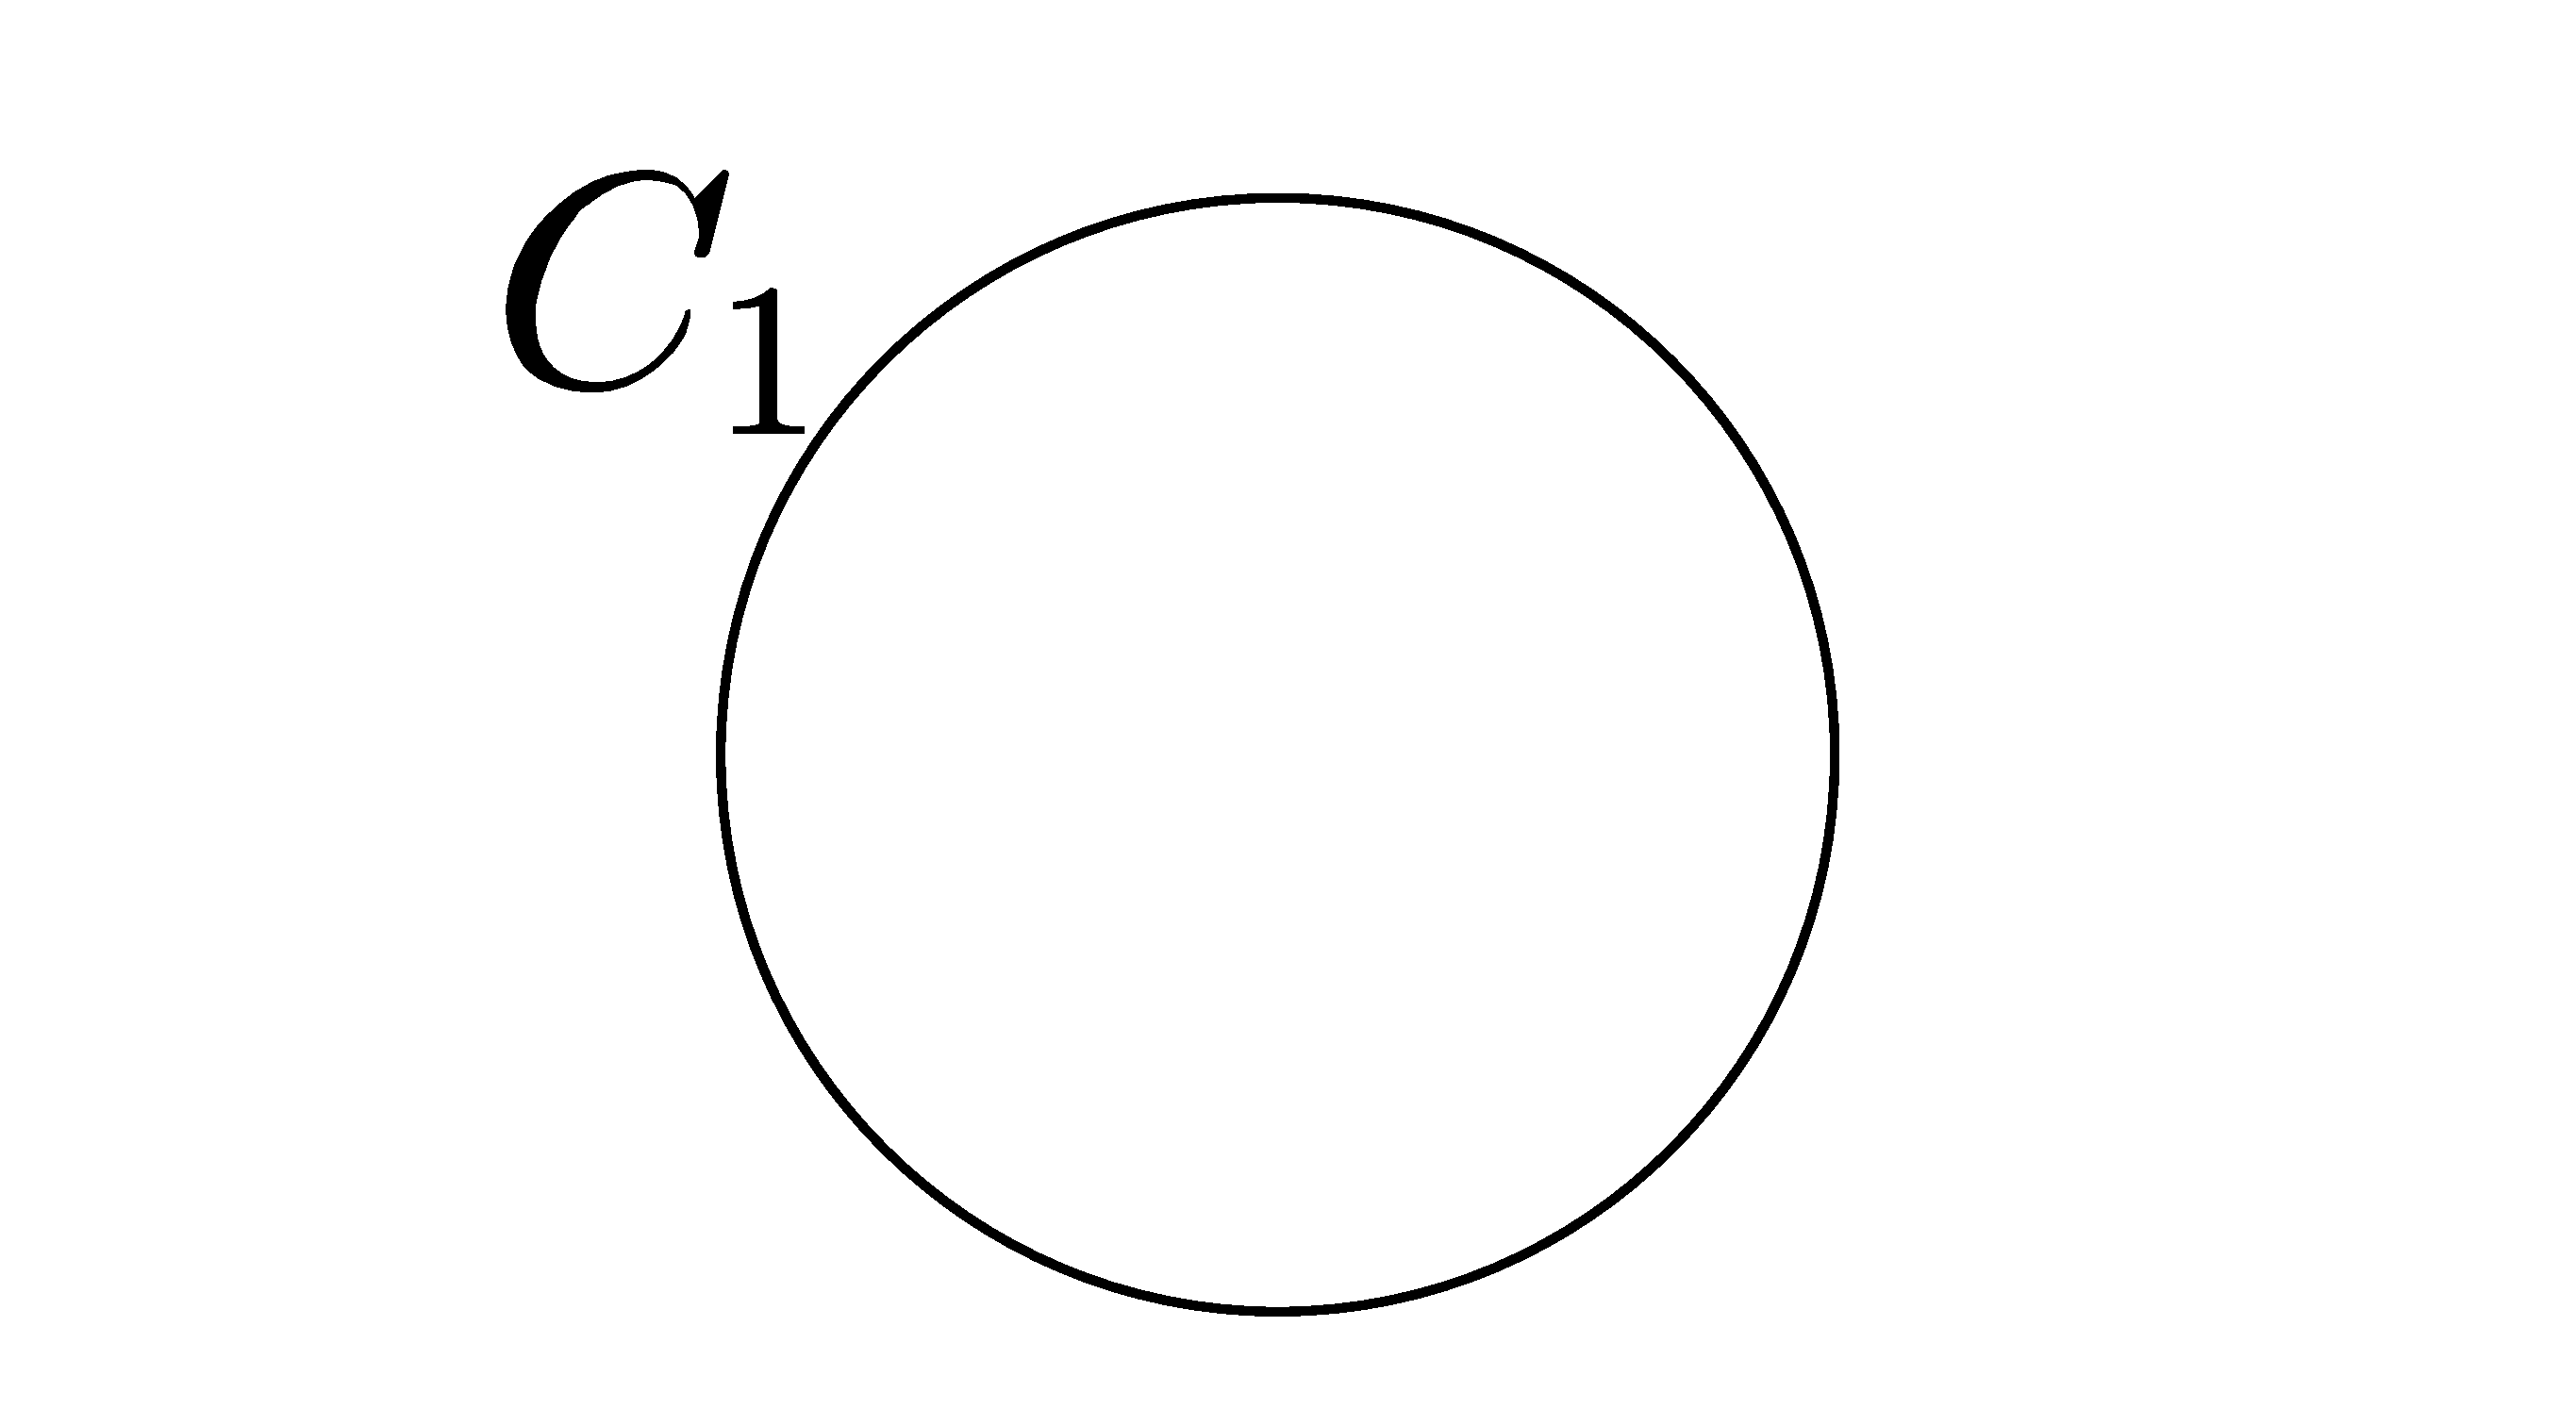
\includegraphics[scale=.065]{Graficos/elipse.eps}}
	\subfigure[Hipérbola]{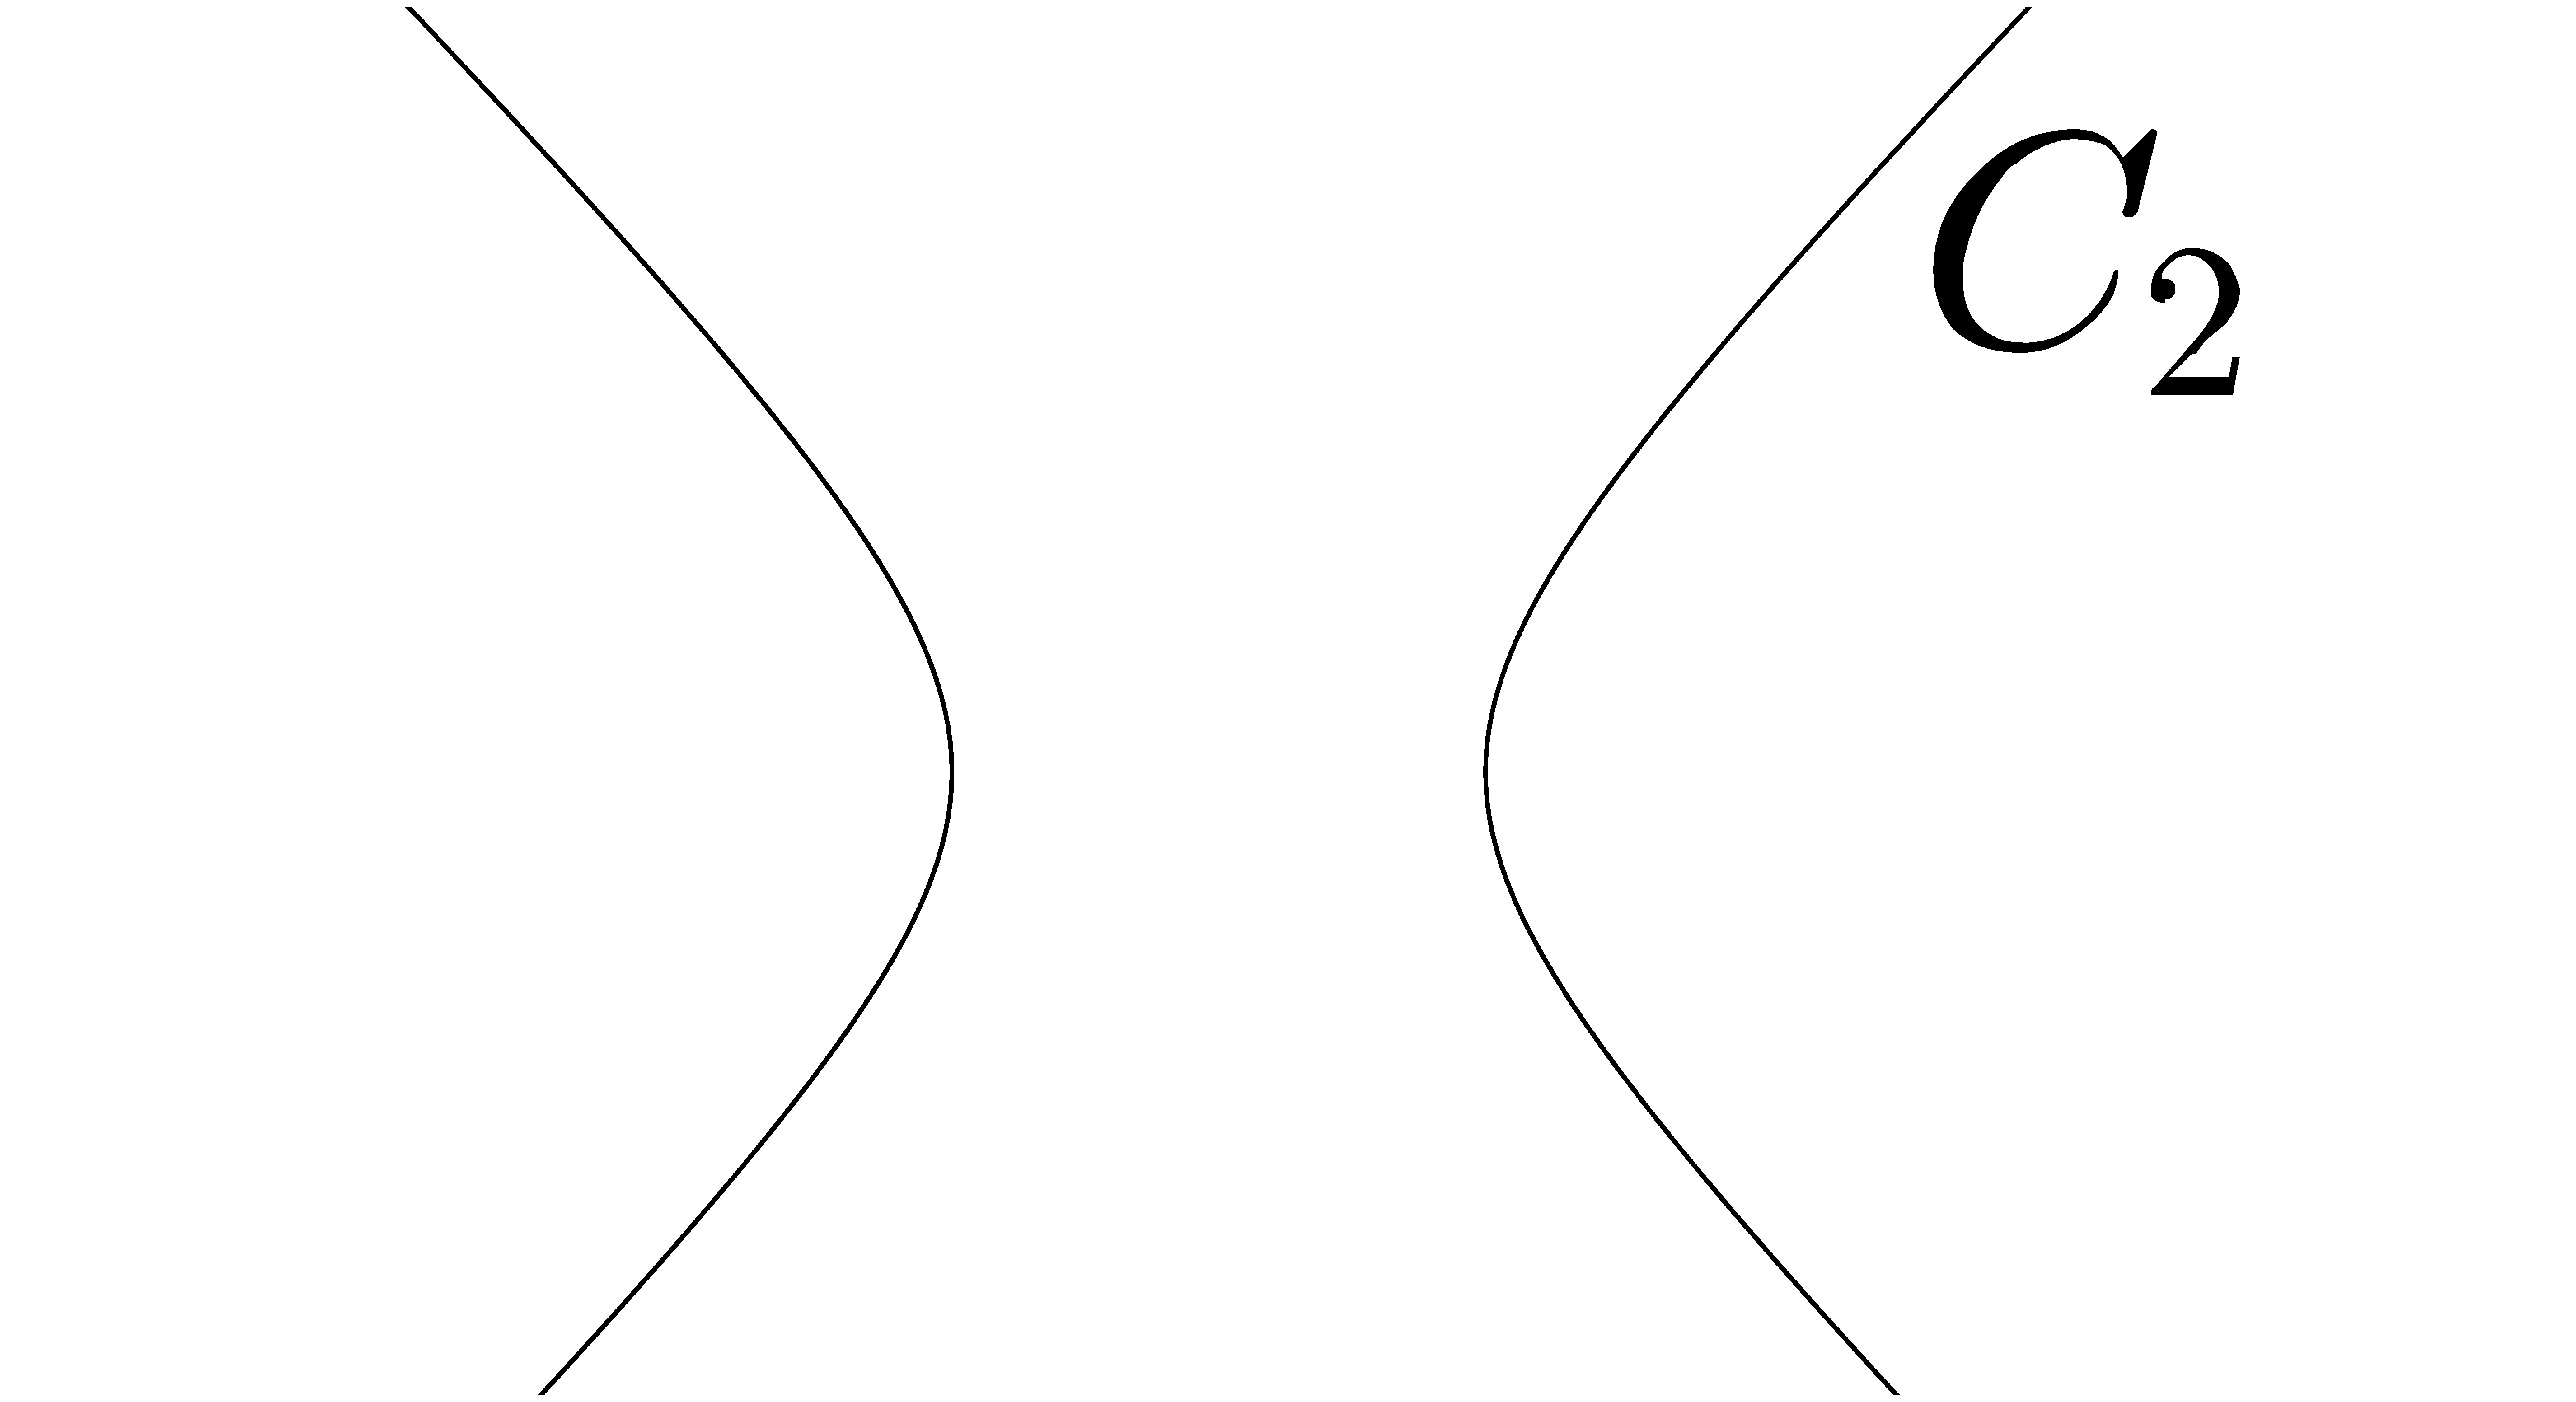
\includegraphics[scale=.028]{Graficos/hiperbola.eps}}
	\subfigure[Parábola]{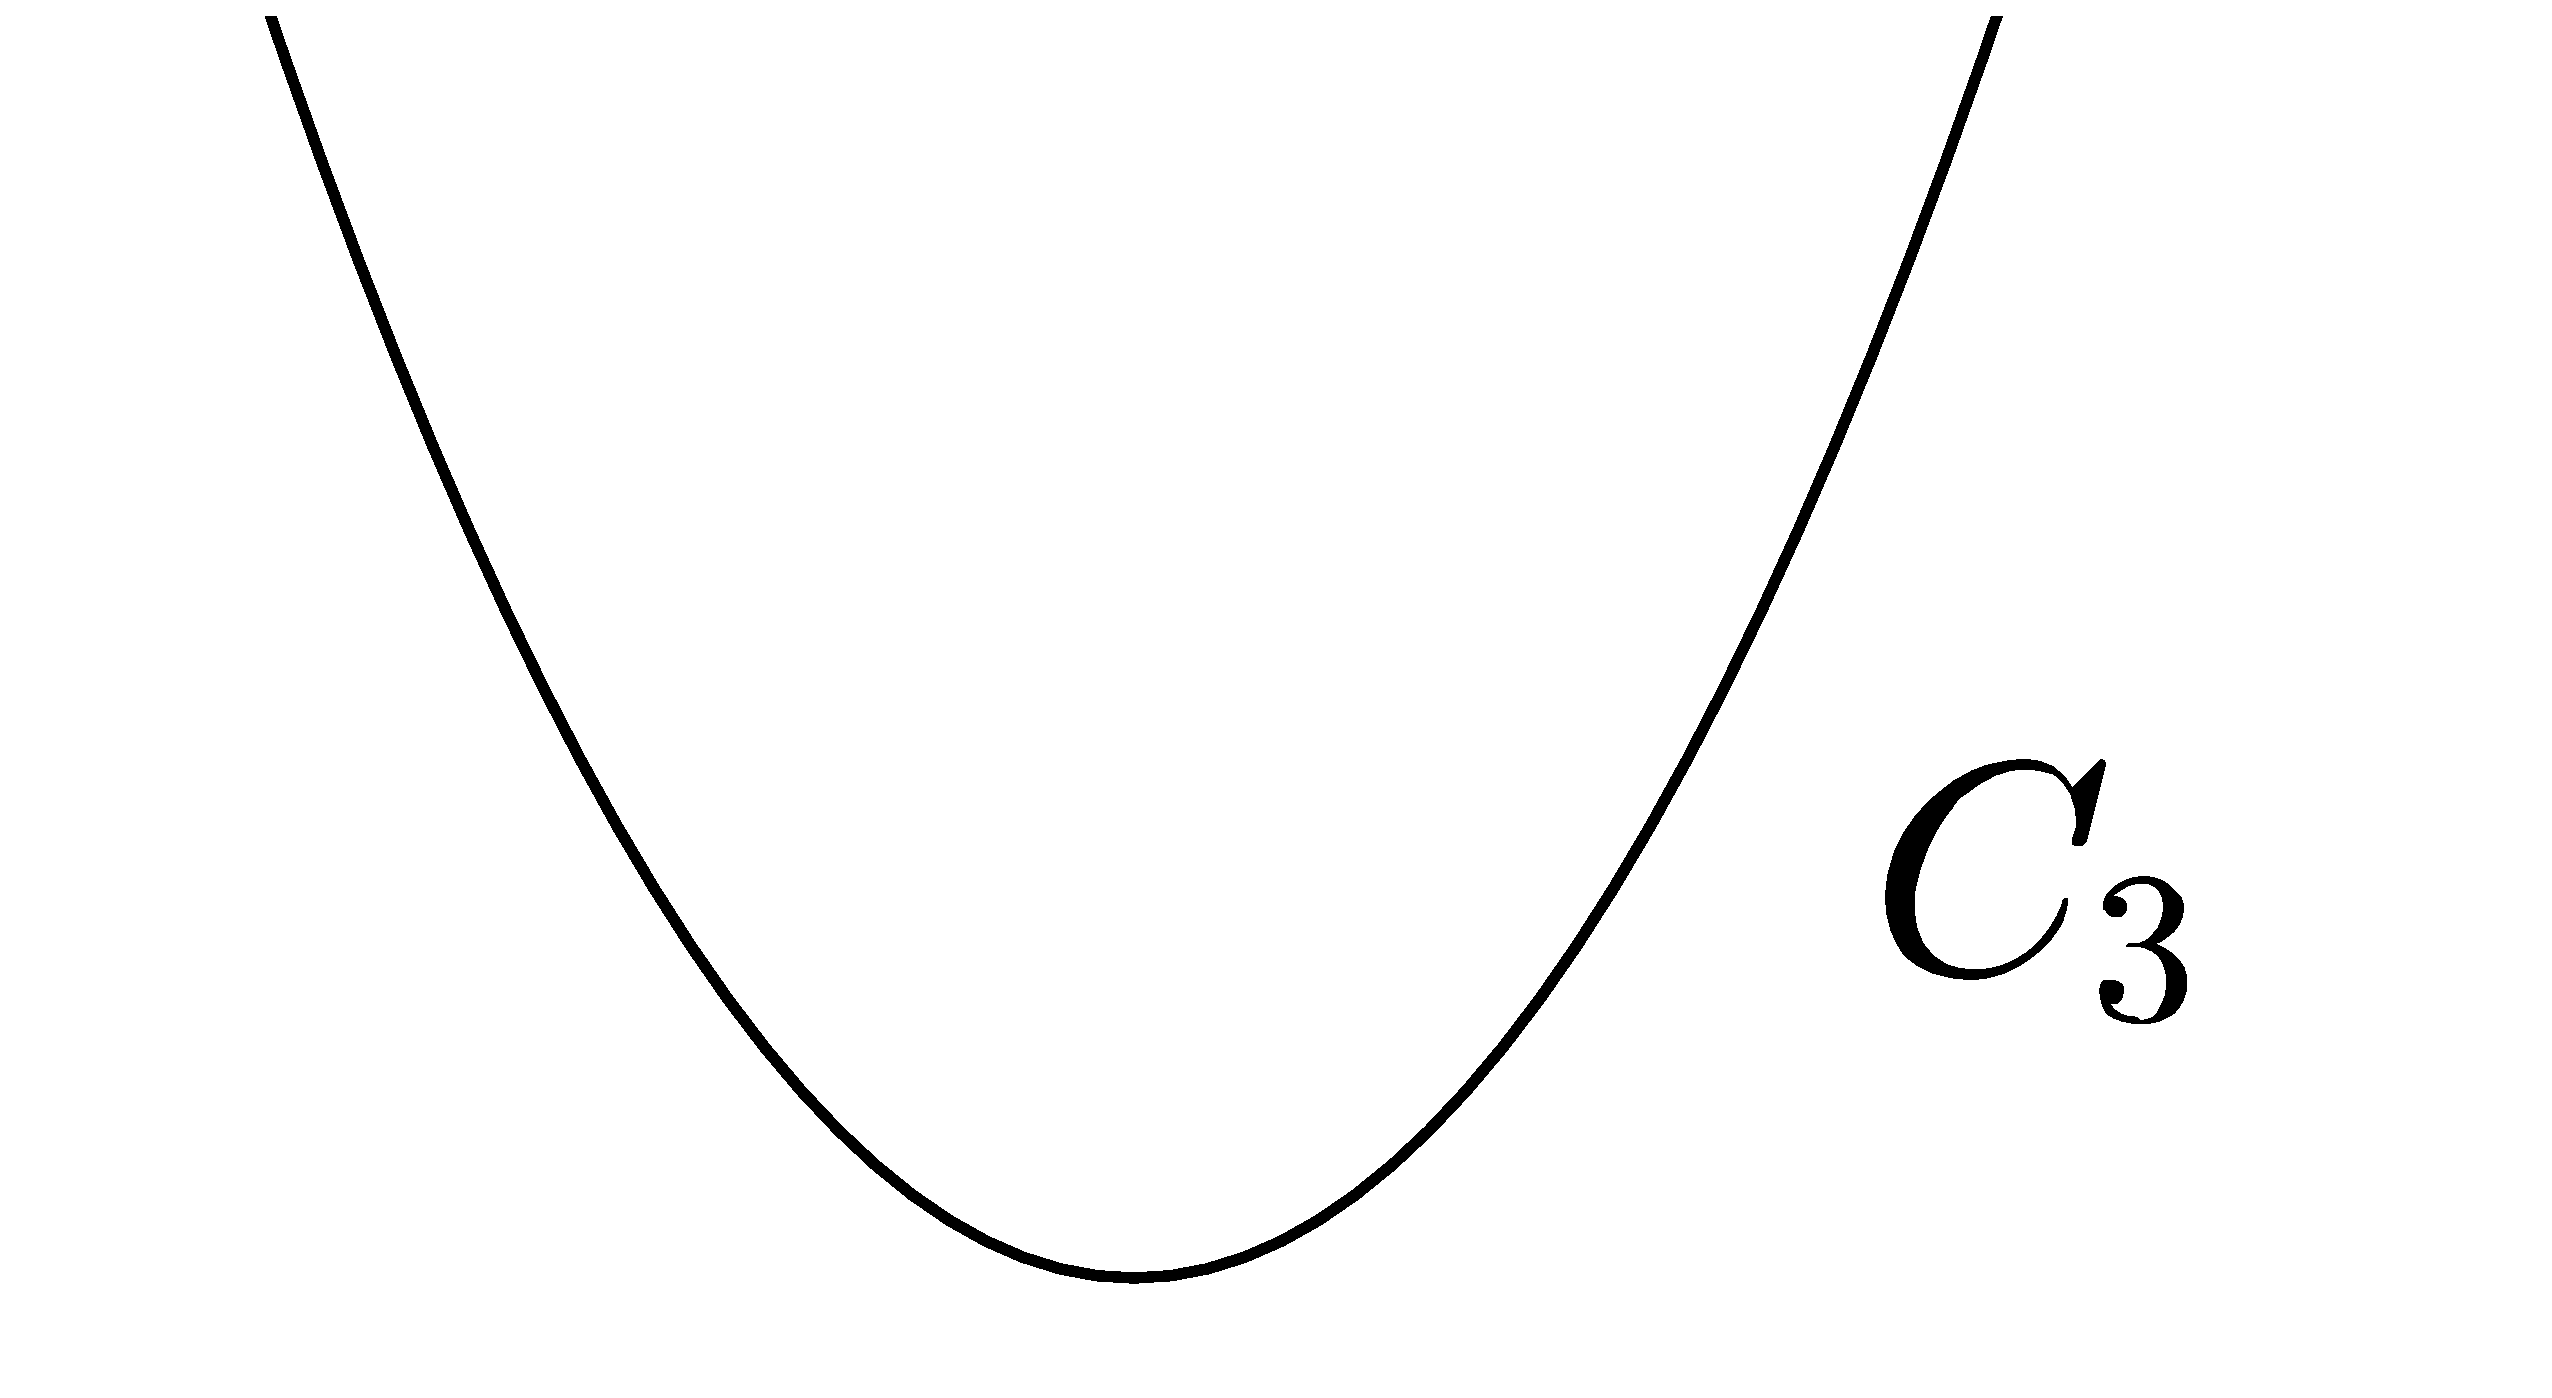
\includegraphics[scale=.06]{Graficos/parabola.eps}}
	\caption{Ilustración de los tipos de cónicas.}
	\label{C7_img_tiposConicas}
\end{figure}
Para que esta clasificación no resulte demasiado abstracta al lector, pongamos un ejemplos de cónicas de cada uno de los tipos.
\begin{exa}[Elipse]
	\label{C8_exa_elipse}
	Consideramos la cónica dada por la siguiente ecuación:
	\[C:x^2+y^2-z^2=0\]
	Intersequemos la cónica con la recta $l_\infty:z=0$ para poder clasificarla.
	\[\left.\begin{array}{c}
	x^2+y^2-z^2=0\\
	z=0
	\end{array}\right\}\leadsto x^2+y^2=0\]
	Es claro que la única solución a esta ecuación es el punto $(0,0,0)$, sin embargo, el rayo engendrado por este vector no está definido. Por ende, no hay ningún rayo (punto proyectivo) de la cónica que sea, a la vez, un rayo de la recta del infinito. Por ende, esta cónica es una elipse.
\end{exa}
\begin{exa}[Hipérbola]
	Clasifiquemos la cónica de ecuación:
	\[C:X^2-Y^2=1\]
	Antes de que cunda el pánico, nótese que esta ecuación nos viene dada en forma ``deshomogeneizada'' (si no no sería la ecuación de una cónica). Al homogeneizarla nos queda algo bastante más familiar:
	\[C:x^2-y^2-z^2=0\]
	Calculemos los puntos de corte con $z=0$:
	\[\left.\begin{array}{c}
	x^2-y^2-z^2=0\\
	z=0
	\end{array}\right\}\leadsto x^2=y^2\]
	Tomando raíces cuadradas y considerando todos los casos necesarios obtemos como soluciones los puntos de la forma:
	\[\begin{array}{cc}
	\class{(\lambda,\lambda,0)}=(1:1:0)\qquad & \qquad \class{(\lambda,-\lambda,0)}=(1:-1:0)
	\end{array}\]
	Por ende, la cónica $C$ tiene dos puntos de corte con la recta del infinito, esto significa que es de tipo hiperbólico.
\end{exa}
\begin{exa}[Parábola]
	Se nos da la siguiente cónica en forma no homogénea:
	\[C:Y=X^2\]
	Calculemos (tras homogeneizar) los puntos de corte de la misma con $l_\infty$.
	\[\left.\begin{array}{c}
	zy-x^2=0\\
	z=0
	\end{array}\right\}\leadsto x^2=0\]
	Teniendo en cuenta esto, los puntos que cumplen las restricciones impuestas por ambas ecuaciones son los de la forma $(0,\lambda,0)$ (los cuales, además, son solución doble). Estos generan un único rayo. Por ende, la cónica y la recta del infinito únicamente se cortan en un punto. Esto es lo mismo que decir que $C$ es una parábola.
\end{exa}
\section{Deshomogeneizaciones de una Cónica}